Below are some key aspects we discussed regarding the dataset and the performance:
\begin{itemize}
    \item \textbf{Data Visualization:}  
    To better understand the distribution of different wine types, we visualize 
    the dataset in both 2D and 3D spaces. The following figures illustrate the 
    feature distribution and potential class separability.
    \begin{figure}[H]
        \centering
        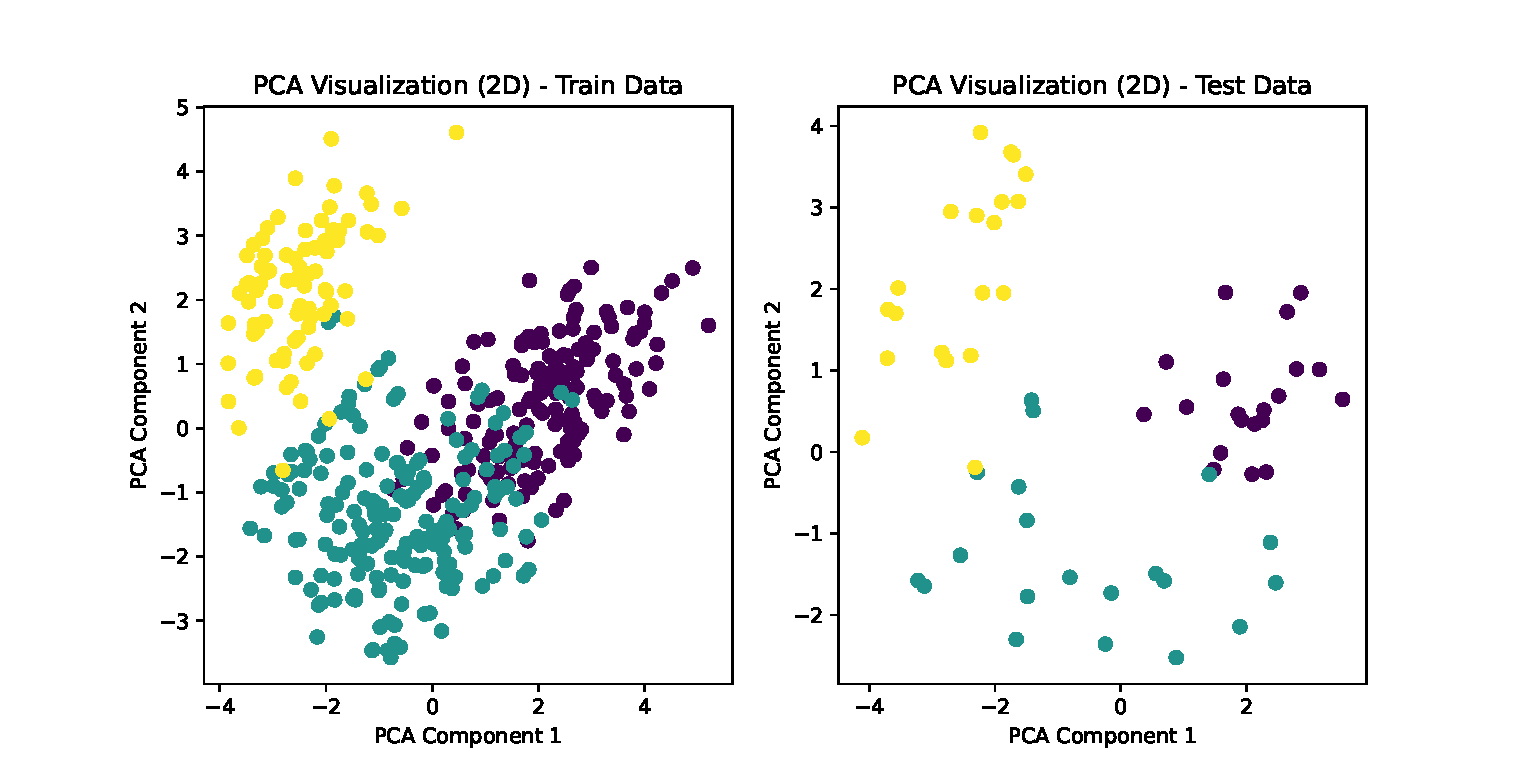
\includegraphics[scale=0.7]{2D_visualize.eps}
        \caption{2D visualization of the dataset.}
        \label{fig:2d_visual}
    \end{figure}
    \begin{figure}[H]
        \centering
        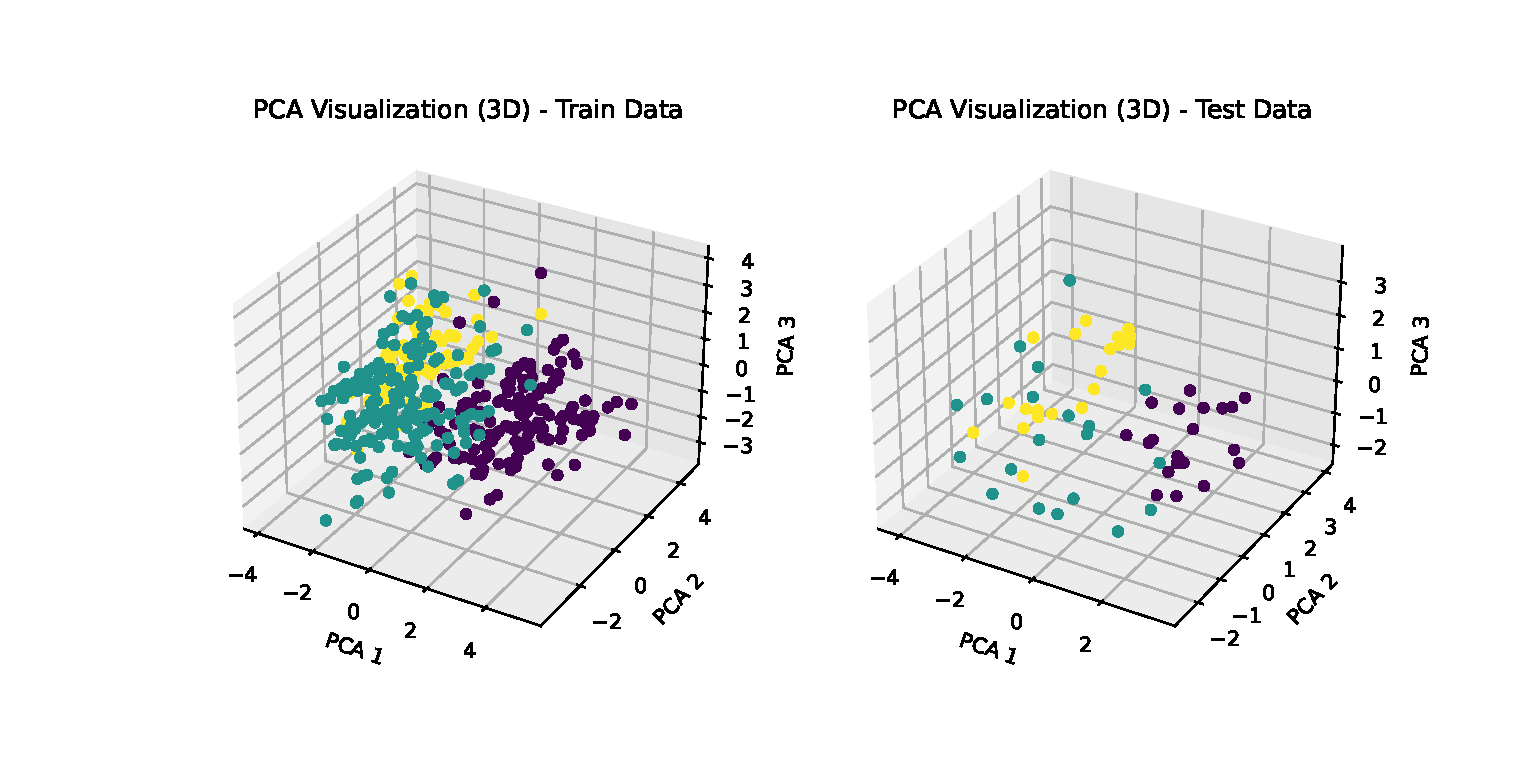
\includegraphics[scale=0.7]{3D_visualize.eps}
        \caption{3D visualization of the dataset.}
        \label{fig:3d_visual}
    \end{figure}
    
    \item \textbf{Effect of Prior Distribution:}  
    To evaluate the influence of prior probabilities on classification performance, 
    we implement a Maximum Likelihood (ML) classifier, which completely disregards 
    prior information. The performance of the ML classifier is shown below:

    \begin{figure}[H]
        \centering
        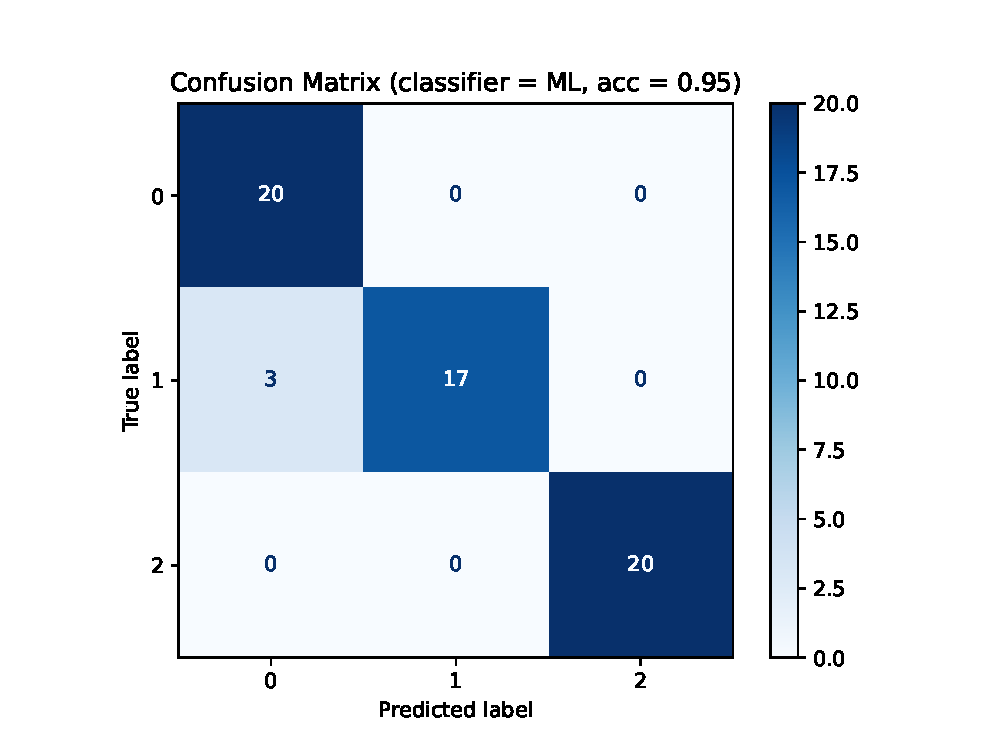
\includegraphics[scale=1.0]{cm_ML.eps}
        \caption{Confusion matrix of the ML classifier.}
        \label{fig:cm_ml}
    \end{figure}

    Interestingly, the results are identical to those obtained with the MAP classifier. 
    This is because, in this problem, the likelihood values are much smaller than the
    prior probabilities. Since the posterior probability is the product of the likelihood 
    and prior, the likelihood becomes the dominant factor, making the effect of the prior 
    negligible.

    \item \textbf{Contribution of Each Feature:} 
    
\end{itemize}
